\documentclass[11pt]{article}

% --- Encoding & fonts -------------------------------------------------------
\usepackage{lmodern}
\usepackage[T1]{fontenc}
\usepackage[utf8]{inputenc}

% --- Layout ----------------------------------------------------------------
\usepackage[margin=1in]{geometry}
\usepackage{microtype}

% --- Math ------------------------------------------------------------------
\usepackage{amsmath}
\usepackage{amssymb}

% --- Graphics & tables -----------------------------------------------------
\usepackage{graphicx}
\usepackage{booktabs}
\usepackage{float}
\usepackage{caption}
\usepackage{xcolor}
\usepackage{pdflscape}
\captionsetup{font=small,labelfont=bf}
\graphicspath{{../figures/}}

% --- Algorithms ------------------------------------------------------------
\usepackage{algorithm}
\usepackage{algpseudocode}

% --- Bibliography ----------------------------------------------------------
\usepackage[round,authoryear]{natbib}
\bibliographystyle{plainnat}

% --- Hyperlinks ------------------------------------------------------------
\usepackage[colorlinks=true,
            linkcolor={blue!55!black},
            citecolor={green!45!black},
            urlcolor={blue!60!black}]{hyperref}

% --- Convenience -----------------------------------------------------------
\newcommand{\sysone}{System~1}
\newcommand{\systwo}{System~2}

\title{\textbf{Thinking, Fast and Slow for Arithmetic:\\
A Dual-Model Agent with Memory for Elementary Multiplication}}
\author{Benjamin Signer\\
\small Undergraduate, Computer Science\\
\small University of California, San Diego}
\date{September 2026}

\begin{document}
\maketitle

\begin{abstract}
\noindent
Large reasoning models solve hard problems reliably but are slow and expensive;
small instruction-tuned models are fast and cheap but unreliable on anything
non-trivial. Inspired by the two-systems account of cognition in Daniel
Kahneman's \emph{Thinking, Fast and Slow}, we build an agentic system that
routes each problem to the cheapest resource likely to solve it correctly. A
fast, non-reasoning ``\sysone'' model answers what it is confident about and
\emph{escalates} the rest, through native tool calls, to a slow, expensive
``\systwo'' reasoning model; a deterministic exact-match memory is consulted
before either model runs. We evaluate the design on a stream of 200 elementary
multiplication problems (with repeats) across four configurations. Confidence
framed routing alone reaches 99.5\% accuracy while sending only 15.5\% of
problems to the reasoning model, at 43\% of the reasoning-only cost. Adding
memory serves 60\% of the stream at zero token cost and drives the full agent to
roughly $6.3\times$ lower cost and $6.5\times$ lower mean latency than the
reasoning-only baseline, for a 0.5 percentage-point accuracy cost (98.5\% vs.\
99.0\%). We report the central trade-off honestly: memory couples correctness to
the quality of the first-contact routing decision, so a confident early mistake
propagates to every repeat. This is an exploratory personal project; we draw
modest conclusions and outline where the design should be pushed next.
\end{abstract}

% ===========================================================================
\section{Introduction}
\label{sec:intro}

In \emph{Thinking, Fast and Slow}, \citet{kahneman2011} describes human thought
as the interaction of two systems: a fast, automatic, low-effort \emph{System~1}
that handles the routine, and a slow, deliberate, effortful \emph{System~2} that
is recruited only when a problem is hard enough to demand it. Crucially, System~1
does not attempt everything; it recognizes when a question exceeds its reach and
hands it off. Much of the efficiency of human cognition comes from this
routing---most of what we do never troubles the expensive machinery at all.

Contemporary language-model deployments face a structurally similar situation.
A small instruction-tuned model is cheap and fast but error-prone; a large
reasoning model is accurate but slow and costly. Using the reasoning model for
\emph{every} query is the machine analogue of engaging effortful deliberation
for $2+2$: correct, but wasteful. This paper asks a simple question:

\begin{quote}
\emph{Can a small model act as a System~1 that decides which problems it can
answer and which it should defer to a larger System~2, and does adding a memory
of previously solved problems yield a system that is substantially cheaper and
faster than always deliberating, without giving up much accuracy?}
\end{quote}

We study this in the deliberately narrow and verifiable domain of elementary
multiplication, where correctness is unambiguous and difficulty is easy to
control. Our contribution is not a new model or a new routing algorithm, but an
honest end-to-end measurement of a Kahneman-inspired agent---which we call
\textbf{TFaS} (Thinking, Fast and Slow)---built from off-the-shelf models, and a
frank account of where memory helps and where it hurts. We deliberately keep the
claims small: this is an exploratory study on a single toy task, intended to
establish the shape of the trade-offs rather than to settle them.

% ===========================================================================
\section{Related Work}
\label{sec:related}

\paragraph{Dual-process theory.} The framing of cognition as two interacting
systems---an intuitive, fast System~1 and a reflective, slow System~2---is
popularized by \citet{kahneman2011}. We borrow the metaphor as an engineering
design principle rather than a cognitive claim: our ``\sysone'' and ``\systwo''
are simply two models with very different cost/accuracy profiles and an explicit
handoff between them.

\paragraph{LLM cascades and routing.} The idea of using a cheap model first and
escalating only when necessary is developed by \citet{chen2023frugalgpt} in
FrugalGPT, which studies LLM ``cascades'' that query a sequence of models and
stop as soon as an answer is deemed good enough, reducing cost while preserving
or improving quality. Our design is a small, concrete instance of this family
with two differences of emphasis: (i) the escalation decision is made by the
small model itself through a native tool call framed around confidence, rather
than by a separate scoring model, and (ii) we add a deterministic memory checked
before any model runs, so repeated problems cost nothing. We do not claim novelty
over the cascade literature; we treat this work as a hands-on replication of the
core idea in a controlled arithmetic setting, with memory added.

% ===========================================================================
\section{System Architecture}
\label{sec:arch}

The full TFaS agent is composed of three components---a memory, a fast \sysone,
and a slow \systwo---connected by a fixed control flow. Both models are served
through the OpenRouter API at temperature~0.

\paragraph{Memory.} Memory is a deterministic exact-match cache keyed by the
ordered problem string (e.g.\ \texttt{"7x8"}). It is consulted \emph{before} any
model call: a hit returns the stored answer immediately, consuming zero tokens.
It is written back after every model-produced answer, whether that answer came
from \sysone{} or \systwo. Because the key is the exact ordered string, the cache
makes no attempt to exploit commutativity ($a\times b = b\times a$) or any other
structure; it only recognizes literal repeats.

\paragraph{\sysone{} (fast).} \sysone{} is \texttt{mistralai/ministral-3b-2512},
a 3-billion-parameter, non-reasoning instruction model
\citep{mistral2024ministral}. Given a problem, it must respond with one of two
\emph{native tool calls}: \texttt{answer(result)} to commit to an integer
answer, or \texttt{escalate()} to defer to \systwo. The prompt is
\emph{confidence-framed}: the model is instructed to answer only when it is
highly confident the result is exactly correct, and otherwise to escalate rather
than guess, on the explicit principle that ``it is much better to escalate than
to give a wrong answer.'' The routing decision is thus genuine self-assessment by
the model, not a hard-coded rule on the number of digits.

\paragraph{\systwo{} (slow).} \systwo{} is
\texttt{deepseek/deepseek-r1-0528}, a larger reasoning model
\citep{deepseek2025r1}. It reasons step by step and then emits a line of the form
\texttt{ANSWER: <integer>}, from which the final answer is parsed. It is
configured with OpenRouter throughput provider routing and a 6000-token budget.

\paragraph{Control flow.} The agent's \texttt{solve()} procedure ties the three
components together, as shown in Algorithm~\ref{alg:solve}: check memory; on a
miss, ask \sysone; if \sysone{} escalates, invoke \systwo; then cache the
model-produced result. Removing components recovers the baselines we compare
against in Section~\ref{sec:setup}: dropping memory and forcing every problem to
\systwo{} gives the reasoning-only baseline, and using only \sysone{} gives the
cheap baseline.

\begin{algorithm}[H]
\caption{\texttt{solve(problem)} --- the full TFaS agent}
\label{alg:solve}
\begin{algorithmic}[1]
\Require problem string $p$ (e.g.\ \texttt{"384x279"})
\If{$p \in \textsc{Memory}$} \Comment{zero tokens on a hit}
    \State \Return $\textsc{Memory}[p]$
\EndIf
\State $(\text{action}, r) \gets \Call{System1}{p}$ \Comment{native tool call: answer or escalate}
\If{$\text{action} = \texttt{answer}$}
    \State $a \gets r$
\Else \Comment{\text{action} $= \texttt{escalate}$}
    \State $a \gets \Call{System2}{p}$ \Comment{step-by-step reasoning}
\EndIf
\State $\textsc{Memory}[p] \gets a$ \Comment{write back for future repeats}
\State \Return $a$
\end{algorithmic}
\end{algorithm}

% ===========================================================================
\section{Experimental Setup}
\label{sec:setup}

\paragraph{Dataset.} We generate a unique pool of 80 multiplication problems: 45
\emph{easy} (single-digit $\times$ single-digit, factors 2--9) and 35 \emph{hard}
(at least one factor with 2--3 digits, a mix of $2d\times1d$, $2d\times2d$,
$3d\times1d$, and $3d\times2d$). From this pool we draw a \emph{stream of 200
problems with repeats}, of which 120 (60\%) are repeated occurrences; the stream
contains 116 easy and 84 hard occurrences. Generation is seeded (seed~0) for
reproducibility. The presence of repeats is what makes memory meaningful, and is
intended to loosely mimic the recurring, over-learned character of the
arithmetic facts that human System~1 answers automatically.

\paragraph{Configurations.} We run four configurations over the identical stream:
\begin{itemize}
  \item \textbf{pure\_system1} --- \sysone{} only, no memory. It must answer
        every problem itself.
  \item \textbf{pure\_system2} --- \systwo{} only, no memory. Every problem is
        deliberated on.
  \item \textbf{hybrid\_no\_memory} --- \sysone{}$\rightarrow$\systwo{} routing,
        no memory. This isolates the value of routing alone.
  \item \textbf{hybrid (TFaS)} --- the full agent: memory
        $\rightarrow$\sysone{}$\rightarrow$\systwo.
\end{itemize}

\paragraph{Metrics.} For each configuration we record accuracy (overall and by
tier), per-problem model latency, wall-clock time, total tokens, USD cost (taken
from OpenRouter's own accounting), the escalation rate (fraction of problems
routed to \systwo), the memory hit rate, and the number of \systwo{} calls.

\paragraph{Infrastructure and concurrency.} All models run through OpenRouter at
temperature~0, and all four runs completed with zero errors. The three stateless
configurations were run concurrently with 12 workers, because \systwo{}
(DeepSeek-R1) exhibits heavy-tailed latency---individual calls ranged from about
12 to 113 seconds---and serial execution would have been needlessly slow. The
memory-enabled hybrid, by contrast, was run \emph{sequentially}: cache
write-backs must be visible to later repeats in the stream for memory to function
as intended. This asymmetry is why the full hybrid's wall-clock time
(Table~\ref{tab:main}) is not comparable to the concurrent runs' wall-clock time
and should be read alongside total latency instead.

% ===========================================================================
\section{Results}
\label{sec:results}

Table~\ref{tab:main} summarizes the four configurations on the curated metrics
that matter most; the complete table with every recorded metric appears in
Appendix~\ref{app:fulltable} (Table~\ref{tab:summary}).

\begin{table}[H]
  \centering
  \caption{Main results: accuracy (overall / easy / hard), mean per-problem
  latency, total tokens, cost, escalation rate, and memory hit rate for each
  configuration over the 200-problem stream. The complete set of metrics is in
  Appendix~\ref{app:fulltable}.}
  \label{tab:main}
  \begin{tabular}{lrrrrrrr}
    \toprule
    \textbf{config} & \textbf{acc.} & \textbf{easy} & \textbf{hard}
      & \textbf{lat.\,(s)} & \textbf{tokens} & \textbf{cost\,(\$)}
      & \textbf{esc.\,/\,mem.} \\
    \midrule
    pure\_system1     & 0.920 & 1.000 & 0.810 &  0.53 &  26{,}113 & 0.0026 & 0.000 / 0.000 \\
    pure\_system2     & 0.990 & 1.000 & 0.976 & 24.14 & 237{,}570 & 0.5282 & 1.000 / 0.000 \\
    hybrid\_no\_memory & 0.995 & 1.000 & 0.988 &  9.39 & 152{,}579 & 0.2272 & 0.155 / 0.000 \\
    hybrid (TFaS)     & 0.985 & 1.000 & 0.964 &  3.74 &  57{,}644 & 0.0835 & 0.060 / 0.600 \\
    \bottomrule
  \end{tabular}
\end{table}

\subsection{Routing alone already pays off}

The clearest result is that confidence-framed routing, with no memory at all,
essentially matches the reasoning-only model at a fraction of its cost.
\texttt{hybrid\_no\_memory} reaches \textbf{99.5\%} overall accuracy---at or
slightly above \texttt{pure\_system2}'s 99.0\%---while sending only \textbf{15.5\%}
(31 of 200) of problems to \systwo. Cost falls to \$0.2272, about \textbf{43\%}
of \texttt{pure\_system2}'s \$0.5282 (Figures~\ref{fig:cost}
and~\ref{fig:route}). In other words, \sysone{} correctly recognized which
problems it could handle---all of the easy tier and most of the hard tier---and
deferred the remainder to the model that could.

\subsection{Memory is the large multiplier}

Adding memory turns a good cost reduction into a large one. Because 60\% of the
stream consists of repeats, the full \texttt{hybrid} answers \textbf{60\%} of
problems directly from cache at zero token cost, escalates only \textbf{6\%} (12
of 200) to \systwo, and costs \textbf{\$0.0835}. Relative to
\texttt{pure\_system2} this is roughly \textbf{$6.3\times$ cheaper}, uses about
\textbf{24\%} of the tokens (57{,}644 vs.\ 237{,}570), and has
\textbf{$6.5\times$ lower} mean latency (3.74\,s vs.\ 24.14\,s), for a
\textbf{0.5 percentage-point} accuracy cost (98.5\% vs.\ 99.0\%). The
accuracy--cost picture is summarized in Figure~\ref{fig:acccost}, and the
divergence of the cumulative-cost curves over the stream in
Figure~\ref{fig:cumcost}: the memory-enabled curve flattens as repeats begin to
be served from cache, while the reasoning-only curve climbs linearly.

\subsection{The extremes}

The two pure baselines frame the trade space. \texttt{pure\_system1} is about
\textbf{$203\times$ cheaper} and \textbf{$46\times$ lower} in mean latency than
\texttt{pure\_system2}, but only \textbf{92.0\%} accurate---and its errors are
concentrated exactly where one would expect, in the hard tier, where it misses
19\% of problems (81.0\% accuracy) despite being perfect on the easy tier
(Figure~\ref{fig:acc}). \texttt{pure\_system2} buys back that hard-tier accuracy
(97.6\%) at two orders of magnitude more cost and latency
(Figures~\ref{fig:latency} and~\ref{fig:tokens}). The hybrids sit in between, and
much closer to the cheap corner than to the expensive one.

% ---- Figures --------------------------------------------------------------
\begin{figure}[t]
  \centering
  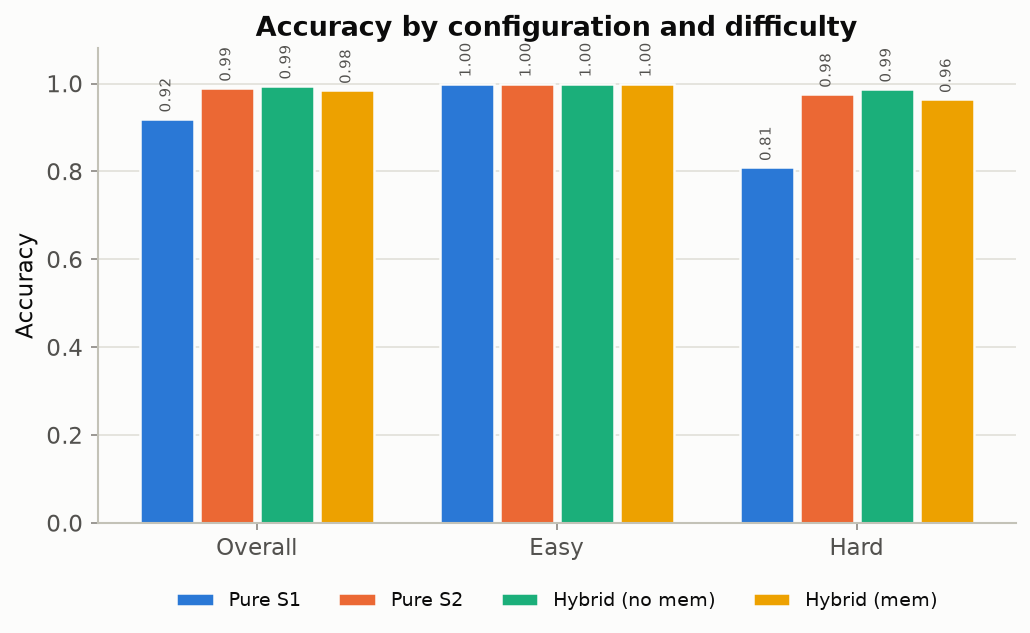
\includegraphics[width=0.78\textwidth]{accuracy_by_config.png}
  \caption{Accuracy by configuration and difficulty tier. All configurations are
  perfect on the easy tier; the differences live entirely in the hard tier,
  where \texttt{pure\_system1} drops to 0.81.}
  \label{fig:acc}
\end{figure}

\begin{figure}[t]
  \centering
  \begin{minipage}[t]{0.48\textwidth}
    \centering
    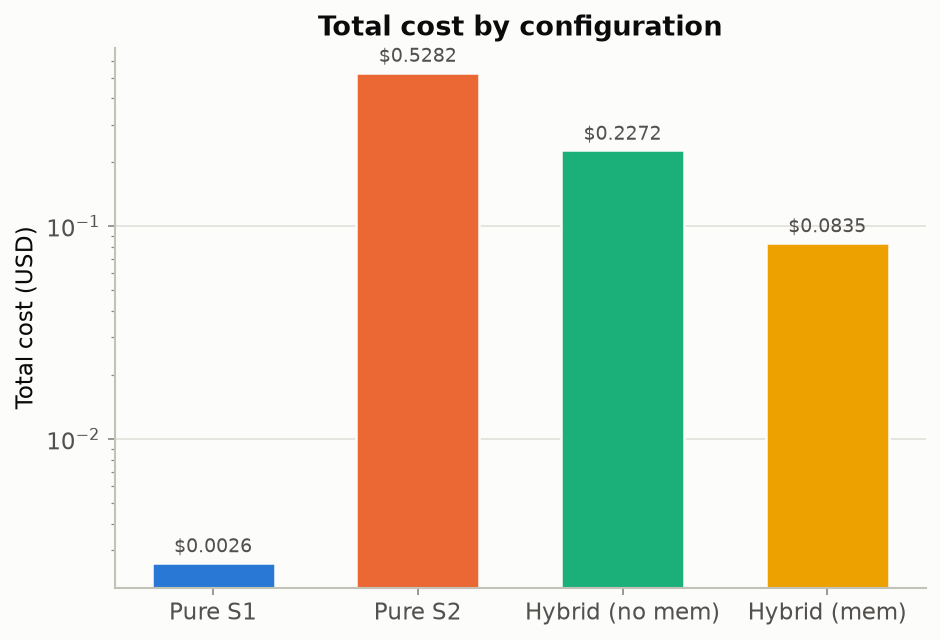
\includegraphics[width=\linewidth]{cost_by_config.png}
    \caption{Total USD cost per configuration (OpenRouter accounting).}
    \label{fig:cost}
  \end{minipage}\hfill
  \begin{minipage}[t]{0.48\textwidth}
    \centering
    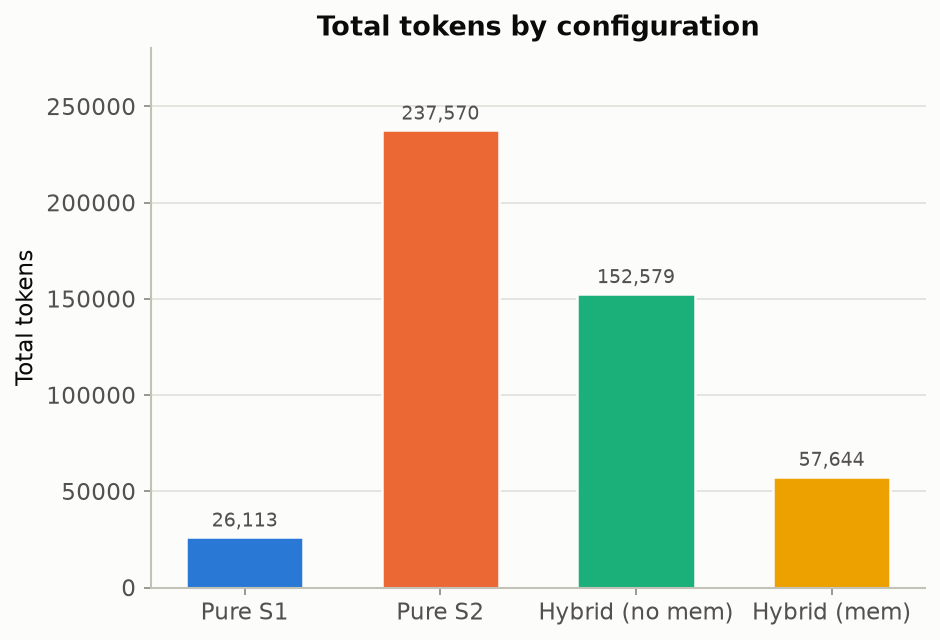
\includegraphics[width=\linewidth]{tokens_by_config.png}
    \caption{Total tokens consumed per configuration.}
    \label{fig:tokens}
  \end{minipage}
\end{figure}

\begin{figure}[t]
  \centering
  \begin{minipage}[t]{0.48\textwidth}
    \centering
    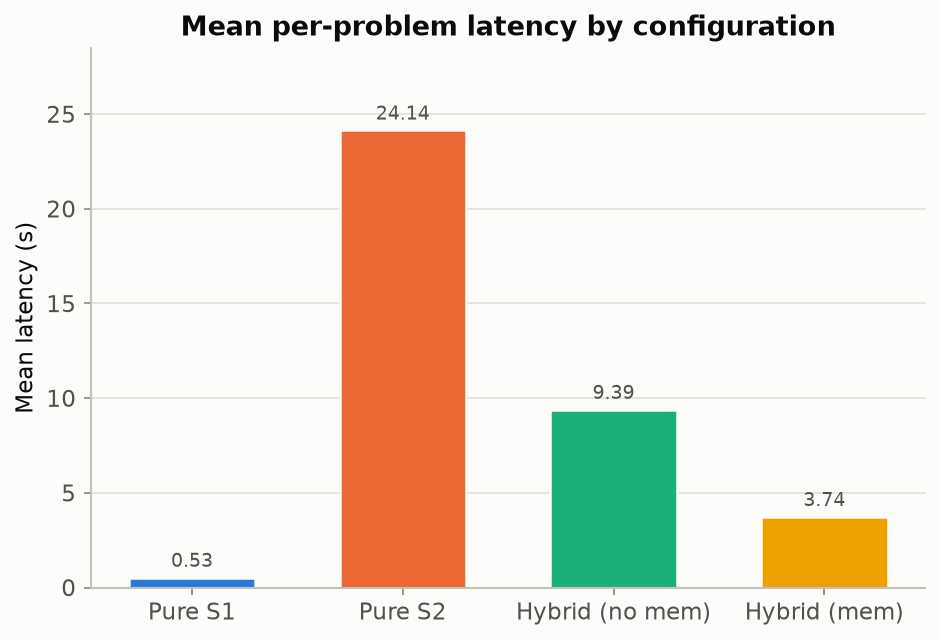
\includegraphics[width=\linewidth]{latency_by_config.png}
    \caption{Mean per-problem model latency per configuration (seconds).}
    \label{fig:latency}
  \end{minipage}\hfill
  \begin{minipage}[t]{0.48\textwidth}
    \centering
    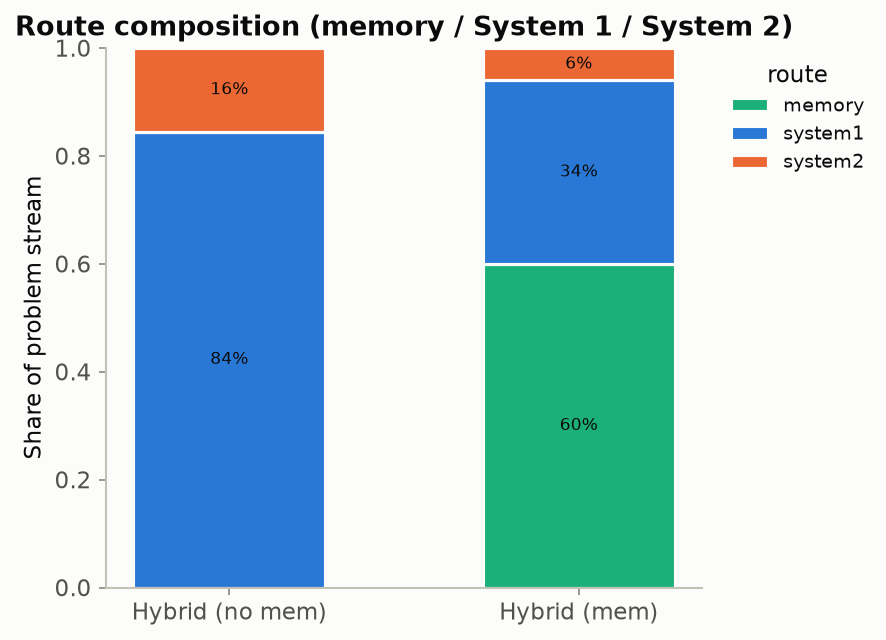
\includegraphics[width=\linewidth]{route_composition.png}
    \caption{Route composition for the two hybrid configurations: the share of
    the stream served by memory, \sysone, and \systwo.}
    \label{fig:route}
  \end{minipage}
\end{figure}

\begin{figure}[t]
  \centering
  \begin{minipage}[t]{0.48\textwidth}
    \centering
    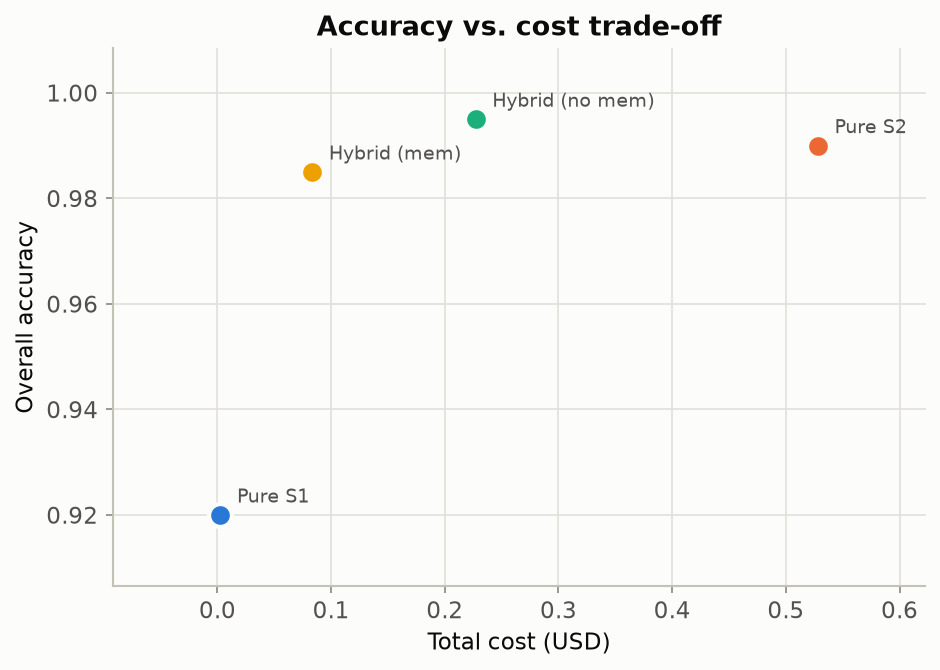
\includegraphics[width=\linewidth]{accuracy_vs_cost.png}
    \caption{Accuracy versus cost---the core trade-off. The hybrids occupy the
    desirable upper-left region.}
    \label{fig:acccost}
  \end{minipage}\hfill
  \begin{minipage}[t]{0.48\textwidth}
    \centering
    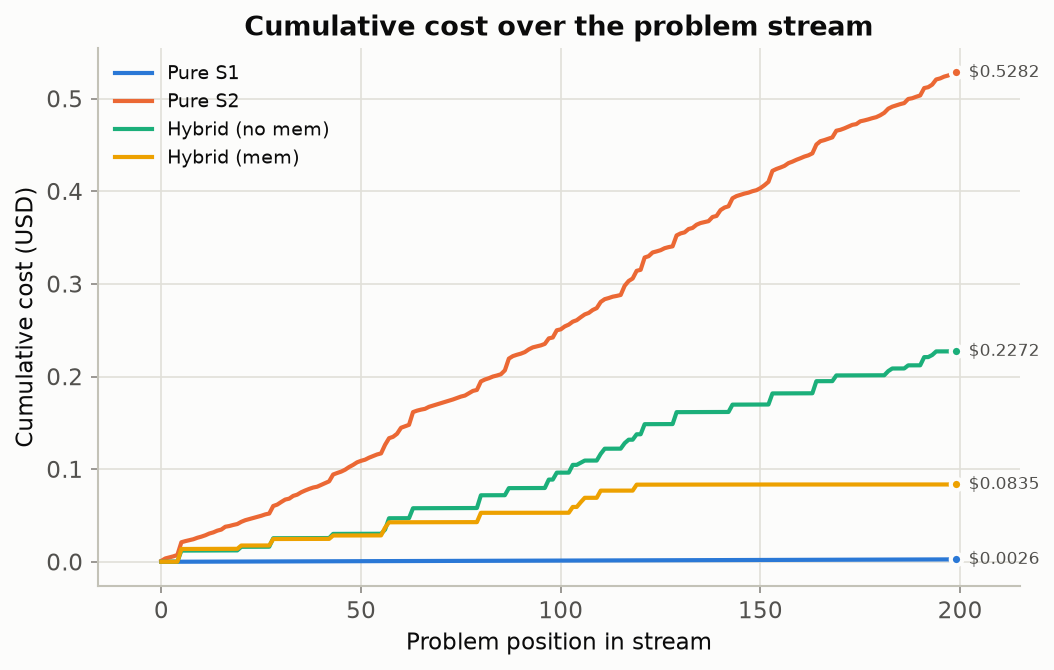
\includegraphics[width=\linewidth]{cumulative_cost.png}
    \caption{Cumulative cost over the problem stream. The memory-enabled hybrid
    flattens as repeats are served from cache.}
    \label{fig:cumcost}
  \end{minipage}
\end{figure}

% ===========================================================================
\section{Discussion}
\label{sec:discussion}

\paragraph{Memory's double edge.} The most important nuance in
Table~\ref{tab:main} is that the full \texttt{hybrid} (98.5\%) is slightly
\emph{below} \texttt{hybrid\_no\_memory} (99.5\%), even though they share the same
router. The cause is structural. Memory caches \sysone{}'s decision on a
problem's \emph{first} occurrence. If \sysone{} is confidently \emph{wrong} on a
hard problem the first time it appears---committing an answer instead of
escalating---that wrong answer is written to the cache and then replayed for
every subsequent repeat, which never gets a fresh chance to escalate to \systwo.
Memory faithfully amplifies the first decision, correct or not. The effect is
compounded by mild provider-side nondeterminism at temperature~0: without memory,
a borderline hard problem can occasionally ``re-roll'' into a correct escalation
on a later occurrence, an escape hatch that memory removes by construction. This
is the central trade-off of the design: memory buys large efficiency gains but
couples end-to-end correctness to the quality of first-contact routing.

\paragraph{Small models need permission to say ``I don't know.''} An early
calibration experiment shaped the whole design. With a naive prompt, the 3B
\sysone{} was \emph{overconfident}: asked for $384\times279$, it answered
$106536$---which is wrong; the correct value is $107136$---instead of escalating.
The model would rather guess than admit uncertainty. Reframing the prompt around
confidence and deference (``it is much better to escalate than to give a wrong
answer'') fixed the routing behavior: the same model then answered $6\times7$ and
$12\times8$ but escalated $23\times47$ and $384\times279$. The lesson is that a
small model's willingness to defer is not automatic; it has to be explicitly
granted. This mirrors the intuition from \citet{kahneman2011} that the value of
System~1 lies as much in knowing its limits as in its speed.

\paragraph{Latency tail.} \systwo's latency was heavy-tailed---individual calls
ranged from roughly 12 to 113 seconds---which is why the reasoning-only mean
latency (24.14\,s) is so much larger than either hybrid's. Every problem routed
away from \systwo{} avoids exposure to this tail, so the latency benefit of
routing and memory is even larger in the worst case than the means suggest. It
also motivated our infrastructure choice to run the stateless configurations
concurrently while keeping the memory hybrid sequential (Section~\ref{sec:setup}).

% ===========================================================================
\section{Limitations and Future Work}
\label{sec:limits}

This is an exploratory study, and its limitations are real.

\begin{itemize}
  \item \textbf{Single, toy task.} We study only elementary multiplication, where
        answers are exactly verifiable and difficulty is trivial to control. Real
        deployments involve open-ended tasks where ``correctness'' and
        ``difficulty'' are far harder to define, and \sysone's self-assessment
        may not transfer.
  \item \textbf{Exact-match memory.} The cache keys on the literal ordered string
        and so ignores commutativity ($7\times8$ and $8\times7$ are distinct
        keys) and generalizes to nothing beyond exact repeats. A semantic or
        approximate memory could capture far more reuse.
  \item \textbf{Modest scale.} A single stream of $N=200$ over a pool of 80 is
        small; the 0.5-point gaps between the strong configurations are within the
        range one would want to confirm with repeated runs and larger streams.
  \item \textbf{Provider variance.} Temperature~0 was not perfectly
        deterministic across provider routing, which contributes noise to the
        comparisons (Section~\ref{sec:discussion}) and complicates exact
        reproduction.
  \item \textbf{No fine-tuning.} Both models are used off the shelf; \sysone's
        routing quality was shaped only by prompting.
\end{itemize}

Natural next steps include a \emph{learned router} (rather than relying on the
small model's self-report), a \emph{semantic or approximate memory} that exploits
commutativity and near-duplicates, extension to \emph{harder task domains} where
verification is nontrivial, and explicit \emph{confidence calibration} of
\sysone{} so that first-contact routing---which we show is the factor memory most
amplifies---is as reliable as possible.

% ===========================================================================
\section{Conclusion}
\label{sec:conclusion}

We built a Kahneman-inspired dual-model agent that routes elementary
multiplication problems to the cheapest resource likely to solve them: a memory
of past answers, a fast \sysone{} that answers what it is confident about, and a
slow \systwo{} for the rest. On a 200-problem stream, confidence-framed routing
alone matched a reasoning-only baseline at 43\% of its cost, and adding memory
made the full agent roughly $6.3\times$ cheaper and $6.5\times$ faster for a
half-point accuracy cost. The same mechanism that delivers those savings---memory
replaying the first decision---also caps accuracy at the quality of first-contact
routing. For an exploratory personal project the takeaway is modest but
clear: a small model, given explicit permission to defer, plus a simple memory,
recovers most of a large model's accuracy at a small fraction of its cost, and
the interesting engineering lies in making that first routing decision good.

% ===========================================================================
\section*{Acknowledgments}
The experiments and this paper were carried out with the assistance of Anthropic's
Claude Opus~4.8, which helped implement the agent and experiment harness, run the
evaluation, and draft the manuscript. The author designed the study, directed the
work, verified the results, and is responsible for all content.

% ===========================================================================
\bibliography{refs}

% ===========================================================================
\appendix
\section{Full Results Table}
\label{app:fulltable}

Table~\ref{tab:summary} reports the complete set of recorded metrics for all four
configurations, laid out with metrics as rows so that every value is legible on a
normal page.

% Requires \usepackage{booktabs} in the document preamble.
\begin{table}[t]
  \centering
  \caption{Full per-configuration results across all recorded metrics. Configurations: Pure S1/S2 use only System~1 / System~2; Hybrid (no mem) is routing without memory; Hybrid (mem) is the full TFaS agent.}
  \label{tab:summary}
  \begin{tabular}{lrrrr}
    \toprule
    \textbf{Metric} & \textbf{Pure S1} & \textbf{Pure S2} & \textbf{Hybrid (no mem)} & \textbf{Hybrid (mem)} \\
    \midrule
    Accuracy (overall) & 0.920 & 0.990 & 0.995 & 0.985 \\
    Accuracy (easy) & 1.000 & 1.000 & 1.000 & 1.000 \\
    Accuracy (hard) & 0.810 & 0.976 & 0.988 & 0.964 \\
    \addlinespace
    Problems ($n$) & 200 & 200 & 200 & 200 \\
    \quad easy & 116 & 116 & 116 & 116 \\
    \quad hard & 84 & 84 & 84 & 84 \\
    \addlinespace
    Mean latency (s) & 0.53 & 24.14 & 9.39 & 3.74 \\
    Total latency (s) & 105.25 & 4828.68 & 1878.78 & 747.13 \\
    Wall-clock (s) & 9.69 & 440.20 & 201.79 & 747.15 \\
    \addlinespace
    Total tokens & 26,113 & 237,570 & 152,579 & 57,644 \\
    Total cost (USD) & 0.0026 & 0.5282 & 0.2272 & 0.0835 \\
    \addlinespace
    Memory hit rate & 0.000 & 0.000 & 0.000 & 0.600 \\
    Escalation rate & 0.000 & 1.000 & 0.155 & 0.060 \\
    System~2 calls & 0 & 200 & 31 & 12 \\
    Errors & 0 & 0 & 0 & 0 \\
    \bottomrule
  \end{tabular}
\end{table}


\section{Reproducibility}
\label{app:repro}

The full pipeline is reproducible from the repository root with three commands
(dataset generation is seeded with seed~0):

\begin{verbatim}
python scripts/generate_dataset.py     # -> data/dataset.json
python scripts/run_experiments.py      # -> results/*.json   (calls the API)
python scripts/make_figures.py         # -> figures/*.png, results/summary_table.tex
\end{verbatim}

The experiment scripts read an OpenRouter API key from the environment
(\texttt{OPENROUTER\_KEY}); a full run costs a few US dollars in OpenRouter
credits. All four configurations reported here completed with zero errors.

\end{document}
